\documentclass[a4paper]{scrartcl}

\usepackage[
    fancytheorems, 
    fancyproofs, 
    noindent, 
]{adam}


\title{Groups, Rings and Modules}
\author{Adam Kelly (\texttt{ak2316@cam.ac.uk})}
\date{\today}

\allowdisplaybreaks

\usepackage{booktabs}

\begin{document}

\maketitle

% This is a short description of the course. It should give a little flavour of what the course is about, and what will be roughly covered in the notes.

In this course we will continue our study of groups, focusing on simple groups, $p$-groups and $p$-subgroups along with the Sylow theorems. We will then move on to discuss rings and fields, finishing up by discussing modules where the scalars belong to a ring instead of a field. 

This article constitutes my notes for the `Groups, Rings and Modules' course, held in Lent 2022 at Cambridge. These notes are \emph{not a transcription of the lectures}, and differ significantly in quite a few areas. Still, all lectured material should be covered.



\tableofcontents

\section{The Theory of Groups}

\subsection{Definition of a Group}

We will begin by recalling the basic definition of a group.


\begin{definition}[Group]
	A \vocab{group} is a pair ($G$, $*$) consisting of a set $G$ and a binary operation $* : G \times G \rightarrow G$ satisfying the axioms:
	\begin{itemize}
		\item \emph{Identity}. There is an element $e \in G$ such that $e * g = g * e = g$ for all $g \in G$,
		\item \emph{Inverses}. For every element $g \in G$, there is an element $g^{-1} \in G$ such that $g * g^{-1} = g^{-1} * g = e$.
		\item \emph{Associativity}. The operation $*$ is associative.
	\end{itemize}
\end{definition}


\begin{remark}
	We will usually either use additive or multiplicative notation for groups, and in these cases we will often write $0$ or $1$ for the identity respectively.
\end{remark}

\begin{definition}[Subgroup]
	A subset $H \subseteq G$ is a \vocab{subgroup} of $G$, written $H \leq G$, if it is a group with respect to the operation $*$ defined on $H \times H$.
\end{definition}

There is a way to test the conditions needed for a subset to be a subgroup in just a few lines, but it does have limited utility.

\begin{lemma}[Fast Subgroup Checking]
A nonempty subset $H \subseteq G$ is a subgroup if $a, b \in H$ implies $a * b^{-1} \in H$.
\end{lemma}
\begin{proof}[Proof Sketch]
	Check that this implies the definition.
\end{proof}

\begin{example}[Examples of Groups]
	The following are all examples of groups.
	\begin{enumerate}[label=(\roman*)]
		\item The additive groups $(\Z, +) \leq (\Q, +) \leq (\R, +)$.
		\item The cyclic group of order $n$, $C_n$.
		\item The dihedral group $D_{2n}$ of the symmetries of a regular $n$-gon.
		\item The symmetric group $S_n$ and alternating group $A_n$, where $S_n$ is the group of permutations of $\{1, 2, \dots, n\}$ and $A_n \leq S_m$ is the group of even permutations. 
		\item The quaternion group $Q_8 = \{\pm 1, \pm i, \pm j, \pm k \}$ with $i^2 = j^2 = k^2 = ijk = -1$.
		\item The matrix groups over some field $F$, $\GL_n(F)$ of all $n \times n$ matrices over $F$ with non-zero determinant, and $\SL_n(F) \leq \GL_n(F)$, the subgroup of matrices with determinant 1.
	\end{enumerate}
\end{example}

\begin{definition}[Direct Product]
	The \vocab{direct product} of groups $G$ and $H$ is $G \times H$ with operation $(g_1, h_1) * (g_2, h_2) = (g_1 g_2, h_1 h_2)$. 
\end{definition}

\subsection{Lagrange's Theorem}

For a subgroup $H \leq G$, the \vocab{left cosets} of $H$ in $G$ are the sets $gH = \{gh \mid h \in H \}$ where $g \in G$. 
The left cosets partition $G$, and it is straightforward to show that each has the same cardinality as $H$. 
These facts immediately give us \emph{Lagrange's theorem}.

\begin{theorem}[Lagrange's Theorem]
  If $G$ is a finite group and $H \leq G$, then
  $$
|G| = |H| \cdot |G : H|,
  $$
  where $|G:H|$ is the \vocab{index} of $H$ in $G$, the number of left cosets of $H$ in $G$.
\end{theorem}

\begin{remark}
  The proof of Lagrange's theorem is equally valid when using right cosets, and as a consequence there is always the same number of left and right cosets for a given subgroup.
\end{remark}

% It is natural to wonder whether there is a converse to Lagrange's theorem, and it turns out that the converse is \emph{not} true in general. There is a partial converse however.

% \begin{theorem}[First Sylow Theorem]
% 	If $G$ is a group with $|G| = p^a m$ where $p$ is a prime and $p \nmid m$, then there exists $H \leq G$ with $|H| = p^a$.
% \end{theorem}

% We will prove this theorem later on.

\begin{definition}[Order of an Element]
	Let $G$ be a group and $g \in G$. 
  The least $n$ such that $g^n = 1$ is the \vocab{order} of $g$. If no such $n$ exists, we say that $g$ has \vocab{infinite order}.
\end{definition}

\begin{remark} 
If $g$ has order $d$, then the division algorithm implies $g^n = 1 \iff d \mid n$. Also by taking powers we can generate a cyclic subgroup of $G$ with $\{1, g, g^2, \dots, g^{d - 1}\} \leq G$, so if $G$ is finite then by Lagrange, $d \mid |G|$.
\end{remark}

% \subsection{Normal Subgroups}

% Recall that a subgroup is normal if it is invariant under conjugation.

% \begin{definition}[Normal Subgroup]
% 	A subgroup $H \leq G$ is \vocab{normal} if $g^{-1} H g = H$ for all $g \in G$. We write $H \normal G$.
% \end{definition}

% The condition of normality is exactly what is needed to be able to form a group from the cosets of a subgroup.

% \begin{proposition}[Quotient Group]
% 	If $H \normal G$, then the set $G/H$ of left cosets of $H$ in $G$ is a group called the \vocab{quotient group} with the operation $g_1 H * g_2 H = (g_1 g_2) H$.
% \end{proposition}
% \begin{proof}
% 	We must check that $*$ is well defined. Suppose that $g_1H = g_1' H$ and $g_2H = g_2' H$. Then $g_1' = g_1 h_1$ and $g_2' = g_2 h_2$ for some $h_1, h_2 \in H$. Then we get $g_1' g_2' H = g_1 h_1 g_2 h_2 H = g_1 h_1 g_2 H$. This is equal to $g_1 g_2 H$ if and only if $(g_1 g_2)^{-1} g_1 h_1 g_2 \in H$, that is, if $g_2^{-1} h_1 g_2 \in H$, which follows from the normality of $H$. Now to check the group axioms, note that associativity is inherited, we have the coset $H$ being the identity, and the inverse of $gH$ being $g^{-1} H$. Thus $G/H$ is a group.
% \end{proof}


\subsection{Homomorphisms and Isomorphisms}

As with many mathematical objects, there are many instances in which we are interested in the structure preserving maps between groups. Such maps are called 
\emph{homomorphisms}.

\begin{definition}[Homomorphism]
  If $G$ and $H$ are groups, a function $\phi: G \rightarrow H$ is a \vocab{group homomorphism} if
  $
  \phi(g_1 g_2) = \phi(g_1) \phi(g_2)
  $
  for all $g_1, g_2 \in G$.
\end{definition}

We frequently care about what elements in the group $H$ can be obtained through this map, and also what elements in $G$ just get sent to the identity. 

\begin{definition}[Kernel]
	The \vocab{kernel} of $\phi$ is $\kernel(\phi) = \{ g \in G \mid \phi(g) = e\}$.
\end{definition}
\begin{definition}[Image]
	The \vocab{image} of $\phi$ is $\image(\phi) = \{ \phi(g) \mid g \in G\}$. 
\end{definition}

It is straightforward to see that $\kernel(\phi) \leq G$ and $\image(\phi) \leq H$.

When we have a homomorphism that gives a bijection between two groups, the groups must have the same underlying algebraic structure. For this reason, we take this to be a notion of two groups being the same.

\begin{definition}[Isomorphism]
  We say that two groups $G$ and $H$ are \vocab{isomorphic} written $G \cong H$ if there is an \emph{isomorphism} between them. That is, if there is a bijective homomorphism $\phi: G \rightarrow H$ between the groups.  
\end{definition}



\subsection{Quotient Groups and the Isomorphism Theorem}


Quotient groups arise naturally in the study of homomorphisms. When we have two groups $G$ and $H$, and some homomorphism $\varphi: G \rightarrow H$, we can see that the elements of $G$ mapping to certain elements of $H$ naturally arrange themselves together.

\begin{center}
	


	\tikzset{every picture/.style={line width=0.75pt}} %set default line width to 0.75pt        

	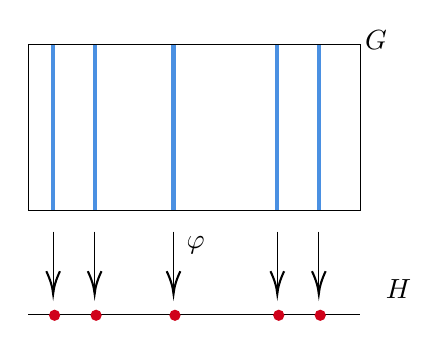
\begin{tikzpicture}[x=0.75pt,y=0.75pt,yscale=-1,xscale=1]
	%uncomment if require: \path (0,300); %set diagram left start at 0, and has height of 300
	
	%Straight Lines [id:da4738114694625044] 
	\draw    (60,170) -- (220,170) ;
	%Straight Lines [id:da11511338342075483] 
	\draw    (130,130) -- (130,158) ;
	\draw [shift={(130,160)}, rotate = 270] [color={rgb, 255:red, 0; green, 0; blue, 0 }  ][line width=0.75]    (10.93,-3.29) .. controls (6.95,-1.4) and (3.31,-0.3) .. (0,0) .. controls (3.31,0.3) and (6.95,1.4) .. (10.93,3.29)   ;
	%Shape: Circle [id:dp33651349641998407] 
	\draw  [draw opacity=0][fill={rgb, 255:red, 208; green, 2; blue, 27 }  ,fill opacity=1 ] (128,170.3) .. controls (128,168.81) and (129.21,167.6) .. (130.7,167.6) .. controls (132.19,167.6) and (133.4,168.81) .. (133.4,170.3) .. controls (133.4,171.79) and (132.19,173) .. (130.7,173) .. controls (129.21,173) and (128,171.79) .. (128,170.3) -- cycle ;
	%Straight Lines [id:da5155967431204146] 
	\draw [color={rgb, 255:red, 74; green, 144; blue, 226 }  ,draw opacity=1 ][line width=1.5]    (130,40) -- (130,120) ;
	%Straight Lines [id:da14331674756217372] 
	\draw    (72,130) -- (72,158) ;
	\draw [shift={(72,160)}, rotate = 270] [color={rgb, 255:red, 0; green, 0; blue, 0 }  ][line width=0.75]    (10.93,-3.29) .. controls (6.95,-1.4) and (3.31,-0.3) .. (0,0) .. controls (3.31,0.3) and (6.95,1.4) .. (10.93,3.29)   ;
	%Shape: Circle [id:dp5096396309384827] 
	\draw  [draw opacity=0][fill={rgb, 255:red, 208; green, 2; blue, 27 }  ,fill opacity=1 ] (70,170.3) .. controls (70,168.81) and (71.21,167.6) .. (72.7,167.6) .. controls (74.19,167.6) and (75.4,168.81) .. (75.4,170.3) .. controls (75.4,171.79) and (74.19,173) .. (72.7,173) .. controls (71.21,173) and (70,171.79) .. (70,170.3) -- cycle ;
	%Straight Lines [id:da9845694947039054] 
	\draw [color={rgb, 255:red, 74; green, 144; blue, 226 }  ,draw opacity=1 ][line width=1.5]    (72,40) -- (72,120) ;
	%Straight Lines [id:da10408362603379395] 
	\draw    (92,130) -- (92,158) ;
	\draw [shift={(92,160)}, rotate = 270] [color={rgb, 255:red, 0; green, 0; blue, 0 }  ][line width=0.75]    (10.93,-3.29) .. controls (6.95,-1.4) and (3.31,-0.3) .. (0,0) .. controls (3.31,0.3) and (6.95,1.4) .. (10.93,3.29)   ;
	%Shape: Circle [id:dp592184874768645] 
	\draw  [draw opacity=0][fill={rgb, 255:red, 208; green, 2; blue, 27 }  ,fill opacity=1 ] (90,170.3) .. controls (90,168.81) and (91.21,167.6) .. (92.7,167.6) .. controls (94.19,167.6) and (95.4,168.81) .. (95.4,170.3) .. controls (95.4,171.79) and (94.19,173) .. (92.7,173) .. controls (91.21,173) and (90,171.79) .. (90,170.3) -- cycle ;
	%Straight Lines [id:da7856952867633485] 
	\draw [color={rgb, 255:red, 74; green, 144; blue, 226 }  ,draw opacity=1 ][line width=1.5]    (92,40) -- (92,120) ;
	%Straight Lines [id:da18609223529659646] 
	\draw    (180,130) -- (180,158) ;
	\draw [shift={(180,160)}, rotate = 270] [color={rgb, 255:red, 0; green, 0; blue, 0 }  ][line width=0.75]    (10.93,-3.29) .. controls (6.95,-1.4) and (3.31,-0.3) .. (0,0) .. controls (3.31,0.3) and (6.95,1.4) .. (10.93,3.29)   ;
	%Straight Lines [id:da005590924400573405] 
	\draw [color={rgb, 255:red, 74; green, 144; blue, 226 }  ,draw opacity=1 ][line width=1.5]    (180,40) -- (180,120) ;
	%Straight Lines [id:da8680905965357972] 
	\draw    (200,130) -- (200,158) ;
	\draw [shift={(200,160)}, rotate = 270] [color={rgb, 255:red, 0; green, 0; blue, 0 }  ][line width=0.75]    (10.93,-3.29) .. controls (6.95,-1.4) and (3.31,-0.3) .. (0,0) .. controls (3.31,0.3) and (6.95,1.4) .. (10.93,3.29)   ;
	%Straight Lines [id:da5630035947767571] 
	\draw [color={rgb, 255:red, 74; green, 144; blue, 226 }  ,draw opacity=1 ][line width=1.5]    (200,40) -- (200,120) ;
	%Shape: Rectangle [id:dp9314276081609332] 
	\draw   (60,40) -- (220,40) -- (220,120) -- (60,120) -- cycle ;
	%Shape: Circle [id:dp7562554584334911] 
	\draw  [draw opacity=0][fill={rgb, 255:red, 208; green, 2; blue, 27 }  ,fill opacity=1 ] (178,170.3) .. controls (178,168.81) and (179.21,167.6) .. (180.7,167.6) .. controls (182.19,167.6) and (183.4,168.81) .. (183.4,170.3) .. controls (183.4,171.79) and (182.19,173) .. (180.7,173) .. controls (179.21,173) and (178,171.79) .. (178,170.3) -- cycle ;
	%Shape: Circle [id:dp9004298600298029] 
	\draw  [draw opacity=0][fill={rgb, 255:red, 208; green, 2; blue, 27 }  ,fill opacity=1 ] (198,170.3) .. controls (198,168.81) and (199.21,167.6) .. (200.7,167.6) .. controls (202.19,167.6) and (203.4,168.81) .. (203.4,170.3) .. controls (203.4,171.79) and (202.19,173) .. (200.7,173) .. controls (199.21,173) and (198,171.79) .. (198,170.3) -- cycle ;
	
	% Text Node
	\draw (221,32) node [anchor=north west][inner sep=0.75pt]    {$G$};
	% Text Node
	\draw (231,152) node [anchor=north west][inner sep=0.75pt]    {$H$};
	% Text Node
	\draw (135,131) node [anchor=north west][inner sep=0.75pt]    {$\varphi $};
	% Text Node
	\draw (100,80) node [anchor=north west][inner sep=0.75pt]    {$\dotsc $};
	% Text Node
	\draw (145,80) node [anchor=north west][inner sep=0.75pt]    {$\dotsc $};
	
	
	\end{tikzpicture}
	
\end{center}


Indeed, if two elements of $G$ map to the same element of $H$ under $\varphi$, we would find that the two elements must differ by an element of the kernel of $\varphi$. So, going back to how the elements of $G$ arrange themselves, it would seem that they are arranged into cosets of the kernel of $\varphi$. It is this observation that leads us to the definition of quotient groups and the isomorphism theorems.


From the discussion above, it is natural to see when we can make the cosets of a given subgroup into another group. It turns out that this only works when we have a specific type of subgroup.

\begin{definition*}[Normal Subgroup]
	We say that a subgroup $N$ of a group $G$ is \vocab{normal} if the left and right cosets coincide, that is, $gN = Ng$ for all $g \in G$. If $N$ is normal in $G$ we write $N \normal G$.
\end{definition*}

Now we can show that the set of cosets of $N$ in $G$, written $G/N$, forms a group.

\begin{theorem*}[Quotient Groups]
	If $N \normal G$, then the set of cosets of $N$ in $G$ forms the \vocab{quotient group} $G/N$ with the operation of coset multiplication, where $gN \cdot g'N = (g g')N$.
\end{theorem*}
\begin{proof}
	We first need to check that coset multiplication is well defined. If we had $a_1 N = a_2N$ and $b_1 N = b_2 N$, then $a_1 = a_2 n_a$ and $b_1 = b_2 n_b$ for some $n_a, n_b \in N$. Then $(a_1 b_1)N = (a_2 n_a b_2 n_b)N = (a_2 b_2)N$, since $N$ is normal in $G$. So our group operation is well defined, and we are just left to check the group axioms.

	We have closure since $g_1 N$ and $g_2N$ being cosets implies $(g_1 g_2)N$ is too. Then we have the identity element $N$, and inverses with $gN \cdot g^{-1}N = N$. Finally we get associativity inherited from $G$, thus we do indeed have a group.
\end{proof}

Now we initially tried to motivate thinking about groups of cosets by noticing that elements in the same coset of the kernel of $\phi$ had the same image. We then used this `normal' property of a subgroup to make this actually work. It turns out that these express the same idea -- normal subgroups are \emph{exactly} the kernels of homomorphisms.

\begin{theorem*}[Kernels are Normal Subgroups]
	If $\phi: G \rightarrow H$ is a homomorphism, then $\ker \phi \normal G$.
\end{theorem*}
\begin{proof}
	We already know that the kernel of a homomorphism is a subgroup, so we just need to check that it is normal. Let $n \in \ker \phi$, and $g \in G$. Then $\phi(gng^{-1}) = \phi(g) \phi(n)\phi(g^{-1}) = \phi(g) \phi(g^{-1}) = e$, thus $gng^{-1} \in \ker \phi$, so $\ker \phi \normal G$ as required.
\end{proof}

\begin{theorem*}[Normal Subgroups are Kernels]
	Given $N \normal G$, the map $\pi: G \mapsto G/N$ with $\pi(g) = gN$ is a surjective homomorphism called the \vocab{quotient map}, and $\kernel \pi = N$. 
\end{theorem*}
\begin{proof}
We first check that $\pi$ is a homomorphism. For $g, h \in G$, we have $\pi(gh) = (gh)N = gN \cdot hN = \pi(g) \pi(h)$ as required. This map is clearly injective, and also $\pi(g) = gN = N \iff g \in N$, so $\ker \pi = N$, as required.
\end{proof}


Looking back again to our original motivation, we can see that the cosets of the kernel seem to form the group that is the image of the homomorphism. This is the exact idea encompassed in quotient groups, and is formalised in the \emph{first isomorphism theorem}.

\begin{theorem*}[First Isomorphism Theorem]
	Let $\varphi:G \rightarrow H$ be a homomorphism. Then $G/\kernel \varphi \cong \image \varphi$.
\end{theorem*}
\begin{proof}
	Consider the map $\op: G/\ker\varphi \rightarrow \image \varphi$ with $g\ker\varphi \mapsto \varphi(g)$. It's easy to see that this is well defined and to check that it's a homomorphism. It's also clearly bijective, and is thus an isomorphism.
\end{proof}

In a sense, this is the way that you should think about normal subgroups and quotient groups -- as the kernels and images of homomorphisms.


\subsection{Isomorphism Theorems}


We now come to the isomorphism theorems.

\begin{theorem}[First Isomorphism Theorem]
	Let $\phi: G \rightarrow H$ be a group homomorphism. Then $\kernel(\phi) \normal G$, and $G/\kernel(\phi) \cong \image(\phi)$.
\end{theorem}
\begin{proof}
	Let $K = \kernel(\phi)$. We already checked that $K \normal G$. Now define $\Phi: G/K \rightarrow \image(\phi)$ by $gK \mapsto \phi(g)$.

	We first check $\Phi$ is well defined and injective. We have
	\begin{align*}
		g_1K = g_2K &\iff g_2^{-1} g_1 \in K \\
		&\iff \phi(g_2^{-1}g_1) = e \\
		&\iff \phi(g_2)^{-1} \phi(g_1) = e  \\
		&\iff \phi(g_1) = \phi(g_2).
	\end{align*}
	Then we check that $\Phi$ is a group homomorphism, with
	\begin{align*}
		\Phi(g_1 K g_2 K) &= \Phi(g_1 g_2 K) \\
			&= \phi(g_1 g_2) \\
			&= \phi(g_1) \phi(g_2) \\
			&= \Phi(g_1 K) \Phi(g_2 K).
	\end{align*}
	Lastly we check that it is surjective. Let $x \in \image(\phi)$, say $x = \phi(g)$ for some $g \in G$. Then $x = \Phi(gK) \in \image(\Phi)$.
\end{proof}

\begin{example}[Using the First Isomorphism Theorem]
	Let $\phi : \C \rightarrow C^{*}$ with $z \mapsto e^z$. As $e^{z + w} = e^z e^w$, this is a group homomorphism from $(\C, +)$ to $(\C^*, \times)$. 

	We find that $\kernel(\phi) = \{ z \in \C \mid e^z = 1 \} = 2 \pi i \Z$, and $\image(\phi) = \C^*$. Thus $\C/2 \pi i \Z \cong \C^*$.
\end{example}

With the first isomorphism theorem, it is not enough to know the statement and proof -- you have to know when to employ it. For example, if asked to prove $\C/2 \pi i \Z \cong \C^*$, you should be able to think of a strategy similar to the one used above.

The first isomorphism theorem is sometimes just called the `isomorphism theorem', and it tends to be more important than the corollaries that we will state.

\begin{corollary}[Second Isomorphism Theorem]
	Let $H \leq G$ and $K \normal G$. Then $HK = \{hk \mid h \in H, k \in K \} \leq G$ and $H \cap K \normal H$, moreover $HK/K \cong H/H \cap K$.
\end{corollary}
\begin{proof}
	Let $h_1 k_1, h_2 k_2 \in HK$. We have
	\begin{align*}
		h_1 k_1 (h_2 k_2)^{-1} &= h_1 k_1 k_2^{-1} h_2^{-1} \\&= h_1 h_2^{-1} h_2 k_1 k_2^{-1} h_2^{-1} \\&= (h_1 h_2^{-1}) (h_2 k_1 k_2^{-1} h_2^{-1}) \in HK,
	\end{align*}
	thus $HK \leq G$, as required.

	Now let $\phi:H \mapsto G/K$ with $h \mapsto hK$. This is the composite of the inclusion $H \hookrightarrow G$ and the quotient map $G \rightarrow G/K$, thus $\phi$ is a group homomorphism.

	We note $\kernel(\phi) = \{h \in H \mid hK = k\} = H \cap K \normal H$, and $\image(\phi) =\{hK \mid h \in H \} = HK / K$. Thus by the first isomorphism theorem,
	$
	H/H \cap K \cong HK/K.
	$
\end{proof}

Before we state the third isomorphism theorem, consider the following motivation. Suppose $K \normal G$. There is a bijection
$$
\{\text{subgroups of } G/K \} \longleftrightarrow \{ \text{subgroups of } G \text{ containing }K \},
$$
obtained by considering the maps $x \mapsto \{g \in G \mid gK \in X \}$ and $H \mapsto H/K$. This restricts to a bijection between 
$$
\{\text{normal subgroups of }G/K \} \longleftrightarrow \{\text{normal subgroups of }G\text{ containing }K\}.
$$

\begin{corollary}[Third Isomorphism Theorem]
	Let $K \leq H \leq G$ be normal subgroups of $G$. Then
	$$
	(G/K) / (H/K) \cong G/H.
	$$
\end{corollary}
\begin{proof}
	Let $\phi: G/K \rightarrow G/H$ with $gK \mapsto gH$. If $g_1K = g_2 K$, then $g_2^{-1}g_1 \in K \leq H$, so $g_1 H = g_2 H$, and thus $\phi$ is well defined. Also $\phi$ is a surjective group homomorphism with kernel $\kernel(\phi) = H/K$. Then apply the first isomorphism.
\end{proof}

\subsection{Simple Groups}

If $K \normal G$, then studying the groups $K$ and the quotient group $G/K$ gives some information about $G$. However, this approach is not always available.

\begin{definition}[Simple Group]
	A group $G$ is \vocab{simple} if $\{e\}$ and $G$ are its only normal subgroups.
\end{definition}

\begin{lemma}[Abelian Simple Groups]
	An abelian group is simple if and only if it is isomorphic to $C_p$ for some prime $p$.
\end{lemma}
\begin{proof}
	By Lagrange's theorem, a subgroup $H \leq C_p$ has order dividing $|C_p| = p$, which is a prime. Hence $H$ has order 1 or $p$, and $H$ is either $\{e\}$ or $H = G$.

	Now let $G$ be an abelian simple group, and $g \in G$ with $g \neq e$. Note that any subgroup of an abelian group is normal, and thus $G$ must have no subgroups other than $G$ and $\{e\}$. But then $G$ has subgroup $\langle g \rangle = \{\dots, g^{-2}, g^{-1}, e, g, g^2, \dots \}$. Since $G$ is simple, this must be the whole group, that is, $G$ is cyclic.

	If $G$ is the infinite cyclic group, then $G \cong (\Z, +)$, which is not simple (as $2 \Z \normal \Z$). Thus $G \cong C_n$ for some $n$. Let $g$ be a generator for $C_n$. If $m \mid n$, then $\langle g^{n/m} \rangle$ is a subgroup of order $m$, but $G$ is simple thus $m = 1$ or $n$, hence $n$ must be prime.
\end{proof}

\begin{lemma}[Composition Series of Finite Groups]
	If $G$ is a finite group then $G$ has a composition series $\{e\} = G_0 \triangleleft G_1 \triangleleft G_2 \triangleleft \cdots \triangleleft G_{m- 1} \triangleleft G_m = G$, with each quotient $G_i / G_{i - 1}$ is simple.

	[Note that $G_i$ need not be normal in $G$.]
\end{lemma}
\begin{proof}
	We induct on $|G|$. If $|G| = 1$ we are done. If $|G| > 1$, then let $G_{m - 1}$ be a normal subgroup of largest possible order (not $|G|$). Then $G/G_{m - 1}$ is simple, and by induction on $G_{m - 1}$, we are done.
\end{proof}


\section{Group Actions}

A useful way to study a group is by studying how it `acts' on some set.
The way we look at this mathematically is through the lense of group actions.

\subsection{Definitions}

We will begin by looking at groups of permutations of a set.

\begin{definition}[$\sym(X)$]
	For a set $X$, let $\sym(X)$ be the group of all bijections $X \rightarrow X$ under composition. We let the identity of this group be $\operatorname{id}$.
\end{definition}

\begin{definition}[Permutation Group]
	A group $G$ is a \vocab{permutation group} (of degree $n$) if $G \leq \sym(X)$ (where $|X| = n$).
\end{definition}

\begin{example}[Examples of Permutation Groups]
	The group $S_n = \sym(\{1, 2, \dots, n\})$ is a permutation group of degree $n$, as is the alternating group $A_n \leq S_n$.

	The group $D_n$, the symmetries of a regular $n$-gon, is a permutation group as it is a subgroup of $\sym(\{\text{vertices of an $n$-gon}\})$.
\end{example}

We can now generalize the notion of a permutation group to the idea mentioned before -- a group acting on a set.
Slightly more useful (and general) than permutation groups is the notion of a group acting on a set.

\begin{definition}[Group Action]
	An action of a group $G$ on a set $X$ is a function $*: G \times X \rightarrow X$ satisfying
	\begin{enumerate}[label=(\roman*)]
		\item $e * x = x$ for all $x \in X$.
		\item $(g_1 g_2) * x = g_1 * (g_2 * x)$ for all $g_2, g_2 \in G$ and $x \in X$.
	\end{enumerate}
\end{definition}

We also think about group actions in the following way, and switching between he points of view can be quite helpful.

\begin{proposition}
	An action of a group $G$ on a set $X$ is equivalent to specifying a group homomorphism $\phi: G \rightarrow \sym(X)$.
\end{proposition}
\begin{proof}
	For each $g \in G$, there is a function $\phi_g : X \rightarrow X$ given by $x \mapsto g * x$. We have $\phi_{g_1 g_2}(x) = (g_1 g_2) * x = g_1 * (g_2 * x) = \phi_{g_1} (\phi_{g_2}(x))$. Thus $\phi_{g_1 g_2} = \phi_{g_1} \circ \phi_{g2}$.
	
	In particular, $\phi_g \circ \phi_{g^{-1}} = \phi_{g^{-1}} \circ \phi_g = \phi_e = \operatorname{id}$. Thus $\phi_g$ is a bijection, and $\phi_g \in \sym(X)$. We define $\phi : G \rightarrow \sym(X)$ with $g \mapsto \phi_g$. Then this is a group homomorphism by the above.
	
	Conversely, let $\phi : G \rightarrow \sym(X)$ be a group homomorphism. Then defining $*: G \times X \rightarrow X$ with $(g, x) \mapsto \phi(g)(x)$, we have that this is a group action since $e * x = \phi(e)(x) = \operatorname{id}(x) = x$ and $(g_1 g_2) * x = \phi(g_1 g_2)(x) = \phi(g_1)(\phi(g_2)(x)) = g_1 * (g_2 * x)$.
\end{proof}

\begin{definition}[Permutation Representation]
	We say $\phi: G \rightarrow \sym(X)$ is a \vocab{permutation representation} of $G$.
\end{definition}

\subsection{Orbits and Stabilisers}

A useful notion is that of \emph{orbits} and \emph{stabilisers}. Informally, the orbit of an element $x$ in a set $S$ acted on by a group $G$ is all of the elements that can be reached by applying elements of $G$. The stabiliser of $x$ is the set of elements in $G$ so that when we apply them, we still have the element $x$.

\begin{definition}[Orbits and Stabilisers]
	Let $G$ act on a set $X$. The \vocab{orbit} of an element $x \in X$ is $\orb_G(x) = \{ g * x \mid g \in G \}$, which is a subset of $X$. The \vocab{stabiliser} of $x \in X$ is $\stab_G(x) = \{ g \in G \mid g * x = x \}$, which is a subgroup of $G$.
\end{definition}

The orbits partition the set $X$. If there is only one orbit then we say that the group action is \vocab{transitive}.
We recall the Orbit-Stabiliser theorem.

\begin{theorem}[Orbit-Stabiliser Theorem]
	There is a bijection between $\orb_G(x)$ and the set of left cosets of $\stab_G(x)$ in $G$. In particular, if $G$ is finite, then
	$$
	|G| = |\orb_G(x)| \cdot |\stab_G(x)|.
	$$
\end{theorem}

\begin{remark}
	The kernel of $\phi$ can be though of as $\kernel \phi = \cap_{x \in X} \stab(X)$ is called the \vocab{kernel of the group action}.
	Also $\stab(g * x) = g \stab(x) g^{-1}$, so if $x, y \in X$ belong to the same orbit then their stabilisers are conjugate subgroups of $G$.
\end{remark}

\subsection{Using Group Actions}

In many cases, the choosing the right group action can help make progress on a problem. With this in mind, it's helpful to have a list of standard group actions that you can apply.

\begin{example}[Examples of Group Actions]
	The following are all group actions.
	\begin{enumerate}[label=(\roman*)]
		\item Let $G$ act on itself by left multiplication, with $g * x = gx$. The kernel of this action is $\{g \in G \mid gx = x \} = \{e\}$, and thus $G$ injects into $\sym(G)$. This proves Cayley's theorem, that any finite group $G$ is isomorphic to a subgroup of $S_n$ for some $n$ (say $n = |G|$).
		\item Let $H \leq G$. Then $G$ acts on the left cosets of $H$ in $G$ by left multiplication. This group action is transitive, with $\stab_H(x) = \{ g \in G \mid gxH = xH \} = xHx^{-1}$. We have the kernel $\ker(\phi) = \bigcap_{x \in G} xHx^{-1}$, which is the largest normal subgroup of $G$ contained in $H$.
		\item Let $G$ act on itself by conjugation, so $g * x = gxg^{-1}$. Here, the orbits and stabilisers are $\orb_G(x) = \{ gxg^{-1} \mid g \in G \} = \ccl_G(x)$, the \vocab{conjugacy class} of $x$ in $G$. The stabilisers are $\stab_G(x) = \{ g \in G \mid gx = xg \} = C_G(x) \leq G$, the \vocab{centraliser} of $x$. The kernel of this action is the \vocab{center}, $Z(G) = \{ g \in g \mid gx = xg \; \forall x \in G \}$.
		
		$G$ also acts by conjugation on any normal subgroup.

		\item Let $X$ be the set of all subgroups of $G$. Then $G$ acts on $X$ by conjugation. That is, $g * H = g H g^{-1} \leq G$. The stabiliser of $H$ is $\{g \in G \mid gHg^{-1} = H \} = N_G(H)$ is the \vocab{normaliser} of $H$ in $G$. This is the largest subgroup of $G$ to contain $H$ as a normal subgroup. In particular $H \normal G \iff N_G(H) = G$. 
	\end{enumerate}
\end{example}

Of this last, the frequently useful actions (that you should readily reach for) are the left multiplication of cosets, conjugation of elements and subgroups.


To see how we can apply group actions to proving a theorem, consider the following result (and mainly it's proof). Here we will use the action of $G$ on the left cosets of a subgroup $H$.

\begin{theorem}
	Let $G$ be a non-abelian simple group, and $H\leq G$ a subgroup of index $n > 1$ in $G$. Then $n \geq 5$ and $G$ is isomorphic to a subgroup of $A_n$.
\end{theorem}
\begin{proof}
	Let $G$ act on $X$, the set of left cosets of $H$ in $G$, by left multiplication, and let $\phi: G \rightarrow \sym(X)$ be the associated permutation representation. Then $\sym(X) = S_n$. As $G$ is simple, we know that $\kernel \phi = \{e\}$ or $G$. If $\kernel \phi = G$, then $\image \phi = \{e\}$, contradicting that $G$ acts transitively on $X$ (since $n > 1$). Thus $\ker \phi$ is trivial, and $G \cong \image \phi \leq S_n$.

	Since $G \leq S_n$ and $A_n \normal S_n$, the second isomorphism theorem gives $G \cap A_n \normal G$ and $G / G \cap A_n \leq S_n / A_n \cong C_2$. But $G$ is simple so $G \cap A_n = \{e\}$ or $G$. If $G \cap A_n = \{e\}$, then $G \hookrightarrow C_2$, which contradicts that $G$ is non-abelian. Otherwise, $G \cap A_n = G$, and $G \leq A_n$. Finally if $n \leq 4$, then $A_n$ has no non-abelian simple subgroups (by listing them), so $n \geq 5$.
\end{proof}

Another example, looking at the rotational symmetries of a icosahedron, is given below.

\begin{example}[Rotational Symmetries of an Icosahedron]
	Let $G$ be the group of rotations of an icosahedron, as pictured.
	\begin{center}
		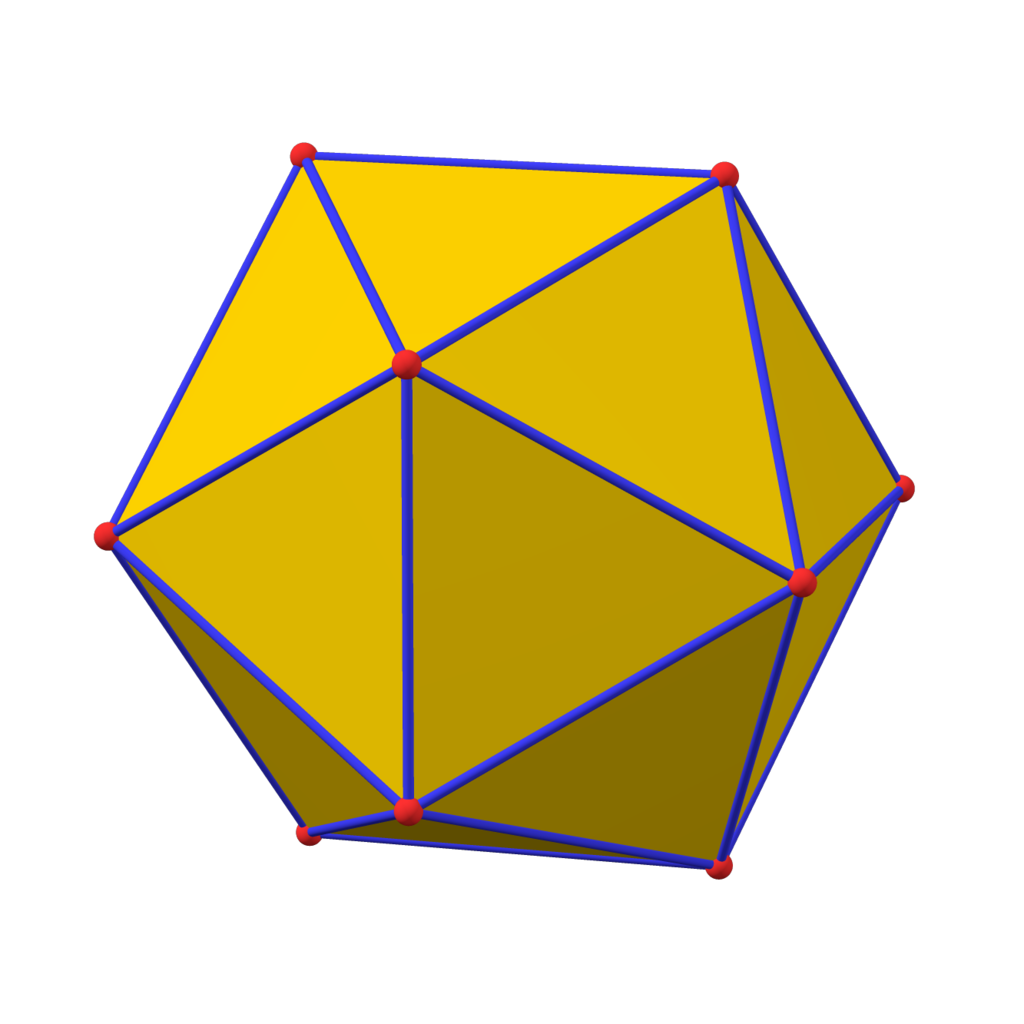
\includegraphics[width=0.25\textwidth]{icosahedron.png}
	\end{center}

	In this shape, there is 20 faces, 12 vertices and 30 edges. We want to know the possible orders of elements in this group, and the number of elements of each order.
\begin{center}
	\begin{tabular}{@{}cc@{}}
		\toprule
		Order & Number of Elements in G   \\ \midrule
		1 	  & 1                         \\
		2	  & 15 \\
		3 	  & 20 \\
		5 	  & 24\\\bottomrule
		\end{tabular}
\end{center}
This gives us a total of $60$ elements. We can verify this with the orbit-stabiliser theorem. For $G$ acting on the vertices, and some vertex $v$, we have $|G| = |\orb(v)| \cdot |\stab(x)| = 12 \cdot 5 = 60$.

To consider the conjugacy classes, we note that two elements are conjugate if they `look the same up to relabelling the icosahedron'.

The elements of order 2 are all conjugate, as are those by order 3. The elements of order 5 split into two conjugacy classes of equal size (12), as the rotations by $\pm \frac{2 \pi}{5}$ are all conjugate and rotations by $\pm \frac{4 \pi}{5}$ are all conjugate, but not to each-other.

We can use this to deduce $G$ is simple. If $H \normal G$, then $|H| = 1 + 15 a + 20b + 12c$ for $a, b \in \{0, 1\}$ and $c \in \{0, 1, 2\}$, but as $|H| \mid 60$ by Lagrange, we get $|H| = 1$ or 60. Thus $G$ is simple.

In fact, $G$ is isomorphic to $A_5$. We will show that the sets $H \leq \{1\}$ for $H \leq G$ a subgroup of order 4 partitions the 15 elements of order 2 into 5 sets of 3. 
\begin{enumerate}
	\item If $|H| = 4$, then $H \cong C_2 \times C_2$ or $H \cong C_4$. But there is no elements of order 4 in $G$, so $H \cong C_2 \times C_2$. Note that this has three elements of order 2.
	\item If $g \in G$ has order 2, then $g \in C_G(g)$ and $|C_G(g)| = \frac{|G||}{|\ccl_G{g}|} = \frac{60}{15} = 4$.
	\item Suppose $e \neq g \in H \cap K$ where $H$ and $K$ are distinct subgroups of order $4$. Then $|C_G(g)| \geq |H \cup K|$ since $H$ and $K$ are abelian, and $|H \cup K| > 4$.
\end{enumerate}
This proves the claim. Now let $G$ act on the set $X$ of subgroups of order 4 by conjugation. We obtain a group homomorphism $\phi:G \rightarrow \sym(X) = S_5$. Then $G$ simple implies either $\kernel \phi = \{e\}$ or $G$. If it was $G$, then we would get that there is a normal subgroup of order $4$m, which is a contradiction. Thus the kernel is trivial, and $G \cong S_5$. Then exactly as before, either $G \cong C_2$ or $G \leq A_5$, and thus $|G| = |A_5| = 60$, so $G \cong A_5$.  
\end{example}

\section{Alternating Groups}

We know from the `Groups' course that two permutations in $S_n$ are conjugate if and only if they have the same cycle type.

\begin{example}[Conjugacy Classes in $S_5$]
	In $S_5$, we have the following:
	\begin{center}
		\begin{tabular}{@{}ccc@{}}
			\toprule
			Cycle Type    & Number of Elements & Sign \\ \midrule
			$1, 1, 1, 1, 1$  & 1   &   $+$  \\ 
			$2, 1, 1, 1$  & 10   &   $-$  \\
			$2, 2, 1$  & 15   &   $+$  \\
			$3, 1, 1$  & 20   &   $+$  \\
			$3, 2$  & 20   &   $-$  \\
			$4, 1$  & 30   &   $-$  \\
			$5$  & 24   &   $+$  \\
			\bottomrule
			\end{tabular}
	\end{center}
	Thus we know the sizes of the conjugacy classes in $S_5$. The same method works in general for $S_n$.
\end{example}

We want to think about the conjugacy classes of $A_n$.

\subsection{Conjugacy Classes \& Simplicity of $A_n$}

One way to think about conjugacy classes is to say that the group acts on itself by conjugation. Then the conjugacy classes correspond to orbits and centralizers correspond to stabilisers.

So it's going to be useful to think about the centralisers of elements in $A_n$. 
Let $g \in A_n$. Then $C_{A_n}(g) = C_{S_n}(g) \cap A_n$. We have then got two cases.
\begin{itemize}
	\item If there exists an odd permutation commuting with $g$, then $|C_{A_n}(g)| = \frac{1}{2}|C_{S_n}(g)|$, and $|\ccl_{A_n}(g)| = |\ccl_{S_n}(g)|$.
	\item  Otherwise, $|C_{A_n}(g)| = |C_{S_n}(g)|$ and $|\ccl_{A_n}(g)| = \frac{1}{2}|\ccl_{S_n}(g)|$.
\end{itemize}

\begin{example}[Conjugacy Classes in $A_5$]
	We can now investigate the conjugacy classes in $A_5$. Note that $(1\ 2)(3\ 4)$ commutes with the odd permutation $(1\ 2)$ and $(1\ 2\ 3)$ commutes with $(4\ 5)$. But if $h \in C_{S_5}(g)$ where $g = (1\ 2\ 3\ 4\ 5)$, then
	$$
(1\ 2\ 3\ 4\ 5) = h (1\ 2\ 3\ 4\ 5) h^{-1} = (h(1)\ h(2)\ h(3)\ h(4)\ h(5)).
	$$
	Thus $h \in \langle g \rangle$, and $|\ccl_{A_5}(g)| = \frac{1}{2}|\ccl_{S_5}(g)| = 12$. Thus $A_5$ has conjugacy classes of size $1, 15, 20, 12, 12$. By the same argument as before, this implies that $A_5$ is simple.
\end{example}

\begin{lemma}[Generators of $A_n$]
	$A_n$ is generated by 3-cycles.
\end{lemma}
\begin{proof}
	We know that each $\sigma \in A_n$ is the product of an even number of transpositions. So it suffices to write the product of any two transpositions as the product of 3-cycles. 

	For $a, b, c, d$ distinct, we have $(a\ b)(b\ c) = (a\ b\ c)$, and $(a\ b)(c\ d) = (a\ c\ b)(a\ c\ d)$.
\end{proof}

\begin{lemma}[3-Cycles are Conjugate in $A_n$]
	If $n \geq 5$, then all $3$-cycles in $A_n$ are conjugate.
\end{lemma}
\begin{proof}
	We claim that every 3-cycle is conjugate to $(1\ 2\ 3)$. Indeed, if $(a\ b\ c)$ is a 3-cycle, then $(a\ b\ c)=\sigma (1\ 2\ 3)\sigma^{-1}$ for some $\sigma \in S_n$. If $\sigma \not \in A_n$, then replace $\sigma$ with $\sigma (4\ 5)$.
\end{proof}

\begin{theorem}[$A_n$ is Simple]
The alternating group $A_n$ is simple for all $n \geq 5$.
\end{theorem}
\begin{proof}
	Let $N \normal A_n$ be a non-trivial subgroup of $A_n$. It suffices to show that $N$ contains a $3$-cycle.
	
	We take some $\sigma \in N$ with $\sigma \neq e$, and write $\sigma$ as the product of disjoint cycles.

	\begin{itemize}
		\item \emph{Case 1}. $\sigma$ contains a cycle of length $r \geq 4$.
	
		Without loss of generality, let $\sigma = (1\ 2\ 3\ \cdots\ r)\tau$. Let $\delta = (1\ 2\ 3)$, then $\delta^{-1} \sigma \delta \in N$, and $\sigma^{-1}\delta^{-1} \sigma \delta \in N$. This can be written $(r\ \cdots\ 2\ 1)(1\ 3\ 2)(1\ 2\ \cdots\ r)(1\ 2\ 3) = (2\ 3\ r)$, which is a three cycle. Then $N$ contains a three cycle.

		\item \emph{Case 2}. $\sigma$ contains two 3-cycles.
		
		Again, without loss of generality say $\sigma = (1\ 2\ 3)(4\ 5\ 6)\tau$. Then let $\delta = (1\ 2\ 4)$, and $\sigma^{-1}\delta^{-1}\sigma \delta = (1\ 3\ 2)(4\ 6\ 5) (1\ 4\ 2)(1\ 2\ 3)(4\ 6\ 5)(1\ 2\ 3) = (1\ 2\ 4\ 3\ 6)$. Then we can apply case 1, and $N$ contains a three cycle.
		\item \emph{Case 3}. $\sigma$ contains two 2-cycles.
		
		Without loss of generality, say $\sigma = (1\ 2)(3\ 4) \tau$. Then let $\delta = (1\ 2\ 3)$. Then $\sigma^{-1}\delta^{-1} \sigma \delta = (1\ 2)(3\ 4)(1\ 3\ 2)(1\ 2)(3\ 4)(1\ 2\ 3) = (1\ 4)(2\ 3)$. Calling this $\pi$, and letting $\epsilon = (2\ 3\ 5)$, then $\pi^{-1} \epsilon^{-1} \pi \epsilon = (1\ 4)(2\ 3)(2\ 5\ 3)(1\ 4)(2\ 3)(2\ 3\ 5) = (2\ 5\ 3)$, so $N$ contains a $3$-cycle. Note that we use $n \geq 5$ here. 
	\end{itemize}
	It remains to consider $\sigma$ where it is a three-cycle. But then $N$ contains a 3-cycle.
\end{proof}

\begin{definition}[Automorphism]
	An \vocab{automorphism} of a group $G$ is an isomorphism $G \rightarrow G$.
\end{definition}

The automorphisms of a group form a subgroup $\aut(G) \leq \sym(G)$.

\section{$p$-Groups and $p$-Subgroups}

\subsection{Basic Properties of $p$-Groups}

Throughout this section, $p$ will denote a fixed prime number.

\begin{definition}[$p$-group]
	A finite group $G$ is a $p$-group if $|G| = p^n$ for $n \in \N$ where $p$ is a prime.
\end{definition}


We will now state some basic properties of $p$-groups that will be used in the following sections.

\begin{theorem}[$p$-groups Have Non-trivial Centers]
	If $G$ is a $p$-group, then $Z(G) \neq \{e\}$.
\end{theorem}
\begin{proof}
	For $g \in G$, we have $|\ccl_G(g)| \cdot |C_G(g)| = |G| = p^n$. So each conjugacy class has size that is a power of $p$. 
	Since $G$ is a union of it's conjugacy classes, 
	\begin{align*}
		|G| &\equiv \#(\text{conj. classes of size 1}) \pmod{p}  \\
\implies 0 &\equiv |Z(G)| \pmod{p}.
	\end{align*}
	In particular, $|Z(g)| > 1$.
\end{proof}

\begin{corollary}[Simple $p$-groups]
	The only simply $p$-group is $C_p$.
\end{corollary}
\begin{proof}
	Let $G$ be a simple $p$-group. Since $Z(G) \normal G$, we have either $Z(G) = \{e\}$ or $G$. The center cannot be trivial by the previous theorem, thus $Z(G) = G$, and the only abelian simple groups are $C_p$.
\end{proof}

\begin{corollary}
	Let $G$ be a $p$-group of order $p^n$. Then $G$ has a subgroup of order $p^r$ for all $0 \leq r \leq n$.
\end{corollary}
\begin{proof}
	We know that any finite group $G$ has a composition series $\{e\} = G_0 \triangleleft G_1 \triangleleft \cdots \triangleleft G_{m - 1} \triangleleft G_m = G$, with each quotient $G_i / G_{i - 1}$ simple. Then $G$ is a $p$-group implies $G_i/G_{i - 1}$ is a $p$-group, and thus $G_i/G_{i - 1} \cong C_p$. Then $|G_i| = p^3$ for all $0 \leq i \leq m$, and $m = n$. 
\end{proof}

\begin{lemma}
	For $G$ a group, if $G/Z(G)$ is cycle, then $G$ is abelian, and $G/Z(G)$ is trivial.
\end{lemma}
\begin{proof}
	Let $gZ(G)$ be a generator for $G/Z(G)$. Then each coset is of the form $g^r Z(G)$ for some $r \in \mathbb{Z}$. Thus $G = \{g^r z \mid r \in \Z, z \in Z(G) \}$.
	Then $(g^{r_1} z_1)(g^{r_2}z_2) = g^{r_1 + r_2} z_1 z_2$ since $z_1$ is in the center.
	We can also write this as $g^{r_1 + r_2}z_2 z_1 =  (g^{r_2} z_2)(g^{r_1} z_1)$, since $z_2$ is also in the center. Thus $G$ is abelian.
\end{proof}

We can now start to consider what various $p$-groups actually look like. We know that a group of order $p$ is cyclic, so we will begin with groups of order $p^2$.

\begin{corollary}[Groups of Order $p^2$]
	If $|G| = p^2$, then $G$ is abelian.
\end{corollary}
\begin{proof}
	The center of $G$ is non-trivial, and by thus by Lagrange, $|Z(G)|$ is either $p$ or $p^2$. If the order was $p^2$, then we would be done. So consider the case $|Z(G)| = p$. Then $|G/Z(G)|$ must have order $p$, but then it is cyclic and contradicts our previous lemma.
\end{proof}

We will leave considering groups of order $p^3$ as an exercise.

\subsection{Sylow Theorems}

Let $G$ be a finite group, and write $|G| = p^a m$ where $p$ is a prime with $p \nmid m$.

\begin{theorem}[First Sylow Theorem]
	The set $\syl_p(G) = \{P \leq G \mid |P| = p^a \}$ of \vocab{Sylow $p$-subgroups} is non-empty.
\end{theorem}
\begin{proof}
	We wish to show that $G$ has a subgroup of order $p^a$.
	Let $\Omega$ be the set of all subsets of $G$ of size $p^a$.
	We have
	$$
	|\Omega| = \binom{p^a m}{p^a} = \frac{p^a m}{p^2} \cdot \frac{p^a m - 1}{p^a - 1} \cdots \frac{p^a m - p^a + 1}{1}.
	$$
	For $0 \leq k < p^a$, the numbers $p^am - k$ and $p^a  -k$ are divisible by the same power of $p$. Thus $|\Omega|$ is coprime to $p$.

	Let $G$ act on $\Omega$ by left multiplication, where for $g \in G
$ and $X \in Omega$, we put $g*X = \{gx \mid x \in X\} \in \Omega$. For any $X \in \Omega$, we have $|\stab_G(X)| \cdot |\orb_G(X)| = |G| = p^a m$. But by the coprimality described above, we can pick $X$ such that $|\orb_G(X)|$ is coprime to $p$. Therefore $p^a \mid |\stab_G(X)|$.

On the other hand, if $g \in G$ and $x \in X$, then $g \in (g x^{-1}) * X$. Therefore $G = \bigcup_{g \in G} g*X$. Thus $|G| \leq |\orb_G(X)| \cdot |X|$, and thus $|\stab_G(X)| = \frac{|G|}{|\orb_G(X)|} \leq |X| = p^a$. So $|\stab_G(X)| = p^a$, and is thus a Sylow $p$-subgroup.
\end{proof}

\begin{theorem}[Second Sylow Theorem]
	All elements of $\syl_p(G)$ are conjugate.
\end{theorem}
\begin{proof}
	We claim that if $P \in \syl_p(G)$ and $Q \leq G$ is a $p$-subgroup then $Q \leq gPg^{-1}$ for some $g \in G$.
	
	Let $Q$ act on the set of left cosets of $G$ by left multiplication, where $q * gP = qgP$. The orbit stabiliser theorem implies each orbit has size dividing $|Q|$, so it is either 1 or a multiple of $p$. 

	Since $|G:P| = m$ is coprime to $p$, there exists an orbit of size 1. Thus there exists $g \in G$ such that $qgP = gP$ for all $q \in Q$, and we get $g^{-1}q g \in P$, so $Q \subseteq gPg^{-1}$.
\end{proof}

\begin{theorem}[Third Sylow Theorem]
	The number $n_p = |\syl_p(G)|$ of Sylow $p$-subgroups satisfies $n_p \equiv 1 \pmod{p}$, and $n_p \mid G$. 
\end{theorem}
\begin{proof}
	Let $G$ act on $\syl_p(G)$ by conjugation. The second Sylow theorem implies that this action is transitive. So by the orbit stabiliser theorem, $n_p = |\syl_p(G)|$ divides $|G|$.

	Now let $P \in \syl_p(G)$. $P$ acts on $\syl_p(G)$ by conjugation. Then the orbits have size dividing $|P|$, so they are either 1 or a multiple of $p$.

	To show $n_p \equiv 1 \pmod{p}$, it suffices to show that $\{P\}$ is the unique orbit of size 1. If $\{Q\}$ is an orbit of size 1, then $P$ normalizes $Q$, so $P \leq N_G(Q)$. Now $P$ and $Q$ are Sylow $p$-subgroups of $N_G(Q)$. Hence by the second Sylow theorem, they are conjugate in $N_G(Q)$, and equal since $Q \normal N_G(Q)$. Thus $\{P\}$ is the unique orbit of size 1.
\end{proof}


\subsection{Applications of the Sylow Theorems}

We will now look at how the Sylow theorems can be use to prove some facts about certain groups.

\begin{corollary}
	If $n_p = 1$, then the unique Sylow $p$-subgroup is normal.
\end{corollary}
\begin{proof}
Let $g \in G$ and $P \in \syl_p(G)$ Then $gPG^{-1} \leq G$ is another Sylow $p$-subgroup, so we must have $gPg^{-1} = P$, for all $g \in G$. Then $P \normal G$.
\end{proof}

\begin{example}[No Simple Groups of Order 1000]
Let $|G| = 1000 = 2^3 \cdot 5^3$. Then $n_5 \equiv 1 \pmod{5}$, and $n_5 \mid 8$. Checking, we find that $n_5 = 1$, and the unique Sylow $5$-subgroup is normal. Then $G$ is not simple.
\end{example}


\begin{example}[No Simple Groups of Order 132]
	Let $|G| = 132 = 2^3 \cdot 3 \cdot 11$. Then $n_{11} \equiv 1 \pmod{11}$, and $n_{11} \pmod 12$. Then $n_{11} = 1$ or $12$. 

	Suppose $G$ was simple. Then $n_{11} \neq 1$, so $n_{11} = 12$. Now $n_3 \equiv 1 \pmod{3}$, and $n_3 \mid 44$, so $n_3 = 1, 4$ or $22$. But $G$ is simple, and either $n_3 = 4$ or $22$. Supposing $n_3 = 4$, then letting $G$ act on $\syl_3(G)$ by conjugation, we get a group homomorphism $\phi: G \rightarrow S_4$. Then $\kernel(\phi) \normal G$ implies $\kernel(\phi) = \{e\}$ or $G$. It cannot be $G$ by the second Sylow theorem, thus $\phi$ is injective. But then $G \hookrightarrow S_4$, and $132 \leq 24$, which is a contradiction.

	Thus $n_3 = 22$, and $n_11 = 12$. But then counting the $G$ has $22 \cdot (3 - 1) = 44$ elements of order 3, and $12 \cdot (11 - 1) = 120$ elements of order 11. But then $120 + 44 = 164 > 132$, which is a contradiction. Thus there does not exist a simple group of order $132$. 
\end{example}

\section{Some Groups}

\subsection{Matrix Groups}

We are going to finish our study of groups by looking at some Matrix groups, along with some finitely generated abelian groups.


Let $F$ be a field (for example $\C$ or $\Z/p\Z$). 
Recall the groups $\GL_n(F)$ of $n \times n$ 
invertible matrices over $F$, and $\SL_n(F) = \kernel(\GL_n \xrightarrow{\det} F^\times) \normal GL_n(F)$.
Also let $Z \normal \GL_n(F)$ be the group of scalar matrices (scalar multiples of the identity matrices). 

We define the \emph{projective general/special linear groups} as follows.

\begin{definition}[Projective General Linear Group]
	The \vocab{projective general linear group} $\PGL_n(F)$ is defined to be $\GL_n(F) / Z$.
\end{definition}

\begin{definition}[Projective Special Linear Group]
	The \vocab{projective special linear group} $\PSL_n(F)$ is the group $\SL_n(F) / (Z \cap  \SL_n(F))$, which is isomorphic to $Z\cdot \SL_n(F) / Z$, by the second isomorphism theorem.
\end{definition}

\begin{example}
	Let $G = \GL_n(\Z/p\Z)$. A list of $n$ vectors in $(\Z/p\Z)^n$ are the columns of some $A \in G$ if and only if they are linearly independent.
	Thus
	\begin{align*}
		|G| &= (p^n - 1)(p^n - p)(p^n - p^2) \cdots (p^n - p^{n - 1}) \\
		&= p^{1 + 2 + \cdots + (n - 1)}(p^n - 1)(p^{n - 1} - 1) \cdots (p - 1) \\
		&= p^{\binom{n}{2}} \prod_{i = 1}^n (p^i - 1).
	\end{align*}

	We see that the Sylow $p$-subgroups have order $p^{\binom{n}{2}}$. One such is the subgroup of upper triangular matrices with 1's on the diagonal.
	$$
	U = \left\{\begin{pmatrix}
		1 & * & * & \cdots & * \\
		0 & 1 & * & \cdots & * \\
		\vdots  &\vdots   & \vdots & \ddots &\vdots \\
		0 & 0 & 0 & \cdots & 1
	\end{pmatrix}\right\} \leq G.
	$$
	Indeed there are $\binom{n}{2}$ entries $*$, each which can take $p$ values, so the order is $p^{\binom{n}{2}}$.
\end{example}

Just as $\PGL_2(\C)$ acts on $\C \cup \{\infty\}$ via Möbius maps, $\PGL_2(\Z/p\Z)$ acts on $\Z/p\Z \cup \{\infty\}$.
Indeed, $\GL_2(\Z/p\Z)$ acts as
$$
\begin{pmatrix}
	a & b\\
	c & d
\end{pmatrix}: z \longmapsto \frac{az + b}{cz + d},
$$
and since scalar matrices act trivially, this is an action of $\PGL_2(\Z/p\Z)$.

\begin{lemma}
	The permutation representation of $\PGL_2(\Z/p\Z) \rightarrow S_{p + 1}$ is injective (and is an isomorphism if $p = 2$ or 3).
\end{lemma}
\begin{proof}
	Suppose $\frac{az + b}{cz + d} = z$ for all $z \in \Z/p\Z \cup \{\infty\}$ Putting $z = 0$ shows $b = 0$. Putting $z = \infty$ shows $c = 0$. Putting $z = 1$ shows $a = d$, and thus this is a scalar matrix. 
\end{proof}

\begin{lemma}
	If $p$ is an odd prime, then $|\PSL_2(\Z/p\Z)| = \frac{p(p - 1)(p + 1)}{2}$.
\end{lemma}
\begin{proof}
	By the previous example, $|\GL_2(\Z/p\Z)| = p(p-1)(p^2 - 1)$. Then consider the group homomorphism $\GL_2(\Z/p\Z) \xrightarrow{\det} (\Z/p\Z)^\times$. This is surjective, since we have
	$$
\begin{pmatrix}
	a & 0 \\
	0 & 1
\end{pmatrix} \longmapsto a,
	$$
	so $|\SL_2(\Z/p\Z)|| = \frac{|\GL_2(\Z/p\Z)|}{p - 1} = p(p - 1)(p + 1)$. 

	Then counting the number of scalar matrices, if
	$$
	\begin{pmatrix}
		\lambda & 0 \\ 0 & \lambda
	\end{pmatrix} \in \SL_2(\Z/p\Z),
	$$
	then $\lambda^2 \equiv 1\pmod{p}$ implies $p \mid (\lambda - 1)(\lambda + 1)$, so $\lambda \equiv \pm 1 \pmod{p}$. So there is two such scalar matrices, and $\PSL_2(\Z/p\Z) = \frac{1}{2}|\SL_2(\Z/p\Z)| = \frac{p(p - 1)(p + 1)}{2}$.
\end{proof}

\begin{example}
	Let $G = \PSL_2(\Z/5\Z)$. Then $|G| = 60 = 2^2 \cdot 3 \cdot 5$.

	Let $G$ act on $\Z/5\Z \cup \{\infty\}$ via Möbius maps. By our previous lemma, there is an injective group homomorphism $\phi : G \rightarrow \sym(\{0, 1, \dots, 4, \infty\}) \cong S_6$.

	\emph{Claim}. $\image(\phi) \leq A_6$, that is, $\psi: G \rightarrow S_6 \xrightarrow{\operatorname{sgn}} \{\pm 1\}$ is trivial.

	If $m$ is odd, then $\psi(g) = e \iff \psi(g)^m = e \iff \psi(g^m) = e$. So it suffices to consider $g \in G$ with order a power of 2. We showed in the proof of the Sylow theorems that every such element belongs to a Sylow 2-subgroup. So it suffices to check that $\psi(H) = e$, where $H$ is a Sylow $2$-subgroup (using that we have any two Sylow $2$-subgroups are conjugate, and $\psi$ maps to an abelian group). 

	We take $H =\left\{ \pm \begin{pmatrix}
		2 & 0 \\ 0 & 3
	\end{pmatrix},\pm \begin{pmatrix}
		0 & 1 \\ -1 & 0 
	\end{pmatrix} \right \} \leq G$. We compute:
	\begin{align*}
		\phi\left(\begin{pmatrix}
			2 & 0 \\ 0 & 3
		\end{pmatrix}\right) &= (1\ 4)(2\ 3)\\
		\phi\left(\begin{pmatrix}
		0 & 1 \\ -1 & 0
		\end{pmatrix}\right) &= (0 \infty)(1\ 4).
	\end{align*} 
	These are even permutations, so $\psi(H)$ is trivial, and our claim is true.
\end{example}

\subsection{Finite Abelian Groups}

Later in this course, we will prove the following theorem.

\begin{theorem}[The Fundamental Theorem of Finite Abelian Groups]
	Every finite abelian group is isomorphic to the direct product of cyclic groups.
\end{theorem}

\begin{remark}[Non-Uniqueness]
	While this is possible, such a decomposition is not unique.
For example, you may recall from IA groups that if $m$ and $n$ are coprime, then $C_m \times C_n \cong C_{mn}$
\end{remark}

\begin{lemma}
	If $m$ and $n$ are coprime, then $C_{mn} = C_m \times C_n$.
\end{lemma}
\begin{proof}
	Let $g$ and $h$ be generators of $C_m$ and $C_n$. Then we have $(g, h) \in C_m \times C_n$, and $(g, h)^r = (g^r, h^r)$. In particular, $(g, h)^r = e$ if and only if $m \mid r$ and $n \mid r$, that is, if $mn \mid r$ since they are coprime. Thus $(g, h)$ has order $mn$, which is $|C_m \times C_n|$.
\end{proof}

\begin{corollary}
	Let $G$ be a finite abelian group.
	Then $G \cong C_{n_1} \times C_{n_2} \times \cdots \times C_{n_k}$ where each $n_i$ is a prime power.
\end{corollary}
\begin{proof}
	If $n = p_1^{a_1} \cdots p_r^{a_r}$, with $p_i$ prime, then we can (by the previous lemma) write $C_{n} \cong C_{p_1^{a_1}} \times \cdots \times C_{p_r^{a_r}}$. Writing each of the cyclic groups in the fundamental theorem of abelian groups then gives the result.
\end{proof}


In fact, we will prove the following refinement of the the fundamental theorem of finite abelian groups.

\begin{theorem}
	Let $G$ be a finite abelian group. Then
	$$
	G \cong C_{d_1} \times C_{d_2} \times \cdots \times C_{d_t},
	$$
	for some $d_1 \mid d_2 \mid \cdots \mid d_t$.
\end{theorem}

\begin{remark}
	The integers $n_1, \dots, n_k$ in the previous corollary and $d_1, \dots, d_t$ in the previous theorem are uniquely determined by $G$.
	The proof (which we omit) works by counting the number of elements of each prime power order.
\end{remark}

\begin{example}[Abelian Groups of Order 8]
	The abelian groups of order 8 are $C_8$, $C_2 \times C_4$ and $C_2 \times C_2 \times C_2$.
\end{example}

\begin{example}[Abelian Groups of Order 12]
	The abelian groups of order 12 are $C_{2} \times C_6 \cong C_2 \times C_2 \times C_3$, $C_4 \times C_3 \cong C_{12}$.
\end{example}

\begin{definition}[Exponent]
	The \vocab{exponent} of a group $G$ is the least integer $n \geq 1$ such that $g^n = e$ for all $g \in G$. That is, it is the lowest common multiple of all of the orders of elements in $G$.
\end{definition}

\begin{example}
	$A_4$ has exponent 6.
\end{example}

\begin{corollary}
	Every finite abelian group contains an element whose order is the exponent of the group.
\end{corollary}
\begin{proof}
	If $G \cong C_{d_1} \times \cdots \times C_{d_t}$ with $d_1 \mid d_2 \mid \cdots \mid d_t$, then every $g \in G$ has order dividing $d_t$, and if $h \in C_{d_t}$ is a generator, then $(1, 1, 1, \dots, h) \in G$ has order $d_t$. So $G$ has exponent $d_t$.
\end{proof}


\section{Rings} 

\subsection{Basic Definitions}



We will now move on to another central algebraic object in this course -- \emph{rings}.
Let's start with a definition.


\begin{definition}[Ring]
	A \vocab{ring} is a triple $(R, +, \cdot)$ consisting of a set $R$ and two binary operations\footnote{Again this has an implicit \emph{closure} axiom} $+, \cdot: \R \times \R \rightarrow R$, refereed to as \emph{addition} and \emph{multiplication}, that satisfy
	\begin{itemize}
		\item $(R, +)$ is an abelian group, with identity $0$.
		\item Multiplication is associative and has an identity $1$.
		\item \emph{Distributivity}. For $x, y, z \in \R$, we have $x \cdot (y + z) = x \cdot y + x \cdot z$ and $(x + y)\cdot z = x \cdot z + y \cdot z$.
	\end{itemize}
\end{definition}

\begin{remark}[Notation]
	For $x \in R$, we write $-x$ for its inverse under addition, and we abbreviate $x + (-y) = x - y$.
\end{remark}

We note that in the definition we require $(R, +)$ to be an abelian group, but the fact that it is abelian is deducible from the other axioms. This means that if we talk about a ring being commutative, we must be referring to the multiplication.

\begin{definition}[Commutative Ring]
	A ring $R$ is \vocab{commutative} if $x \cdot y = y \cdot x$ for all $x, y \in R$.
\end{definition}

In this course, we will \emph{only consider} commutative rings. So whenever we refer to an arbitrary ring, we will be referring to a commutative ring.\footnote{There are some notable non-commutative rings such as ones made up of matrices, but they will not be considered in this course.}


% We can begin to prove some basic facts about rings.

% \begin{proposition}[Basic Properties of Rings]
% 	For a ring $R$, 
% 	\begin{enumerate}
% 		\item $0 \cdot x = 0$ for all $x \in R$.
% 		\item $(-1) \cdot x = -x$ for all $x \in R$.
% 	\end{enumerate}
% \end{proposition}
% \begin{proof}
% 	For the first claim, we have $0 \cdot x = (0 + 0) \cdot x = 0 \cdot x + 0\cdot x$, so we must have $0 \cdot x = 0$.
% 	For the second claim, note that $0 = 0 \cdot x = (1 - 1) \cdot x = 1 \cdot x + (-1) \cdot x = x + (-1) \cdot x$, so $(-1) \cdot x = -x$.
% \end{proof}

We can define subrings in the natural way.

\begin{definition}[Subrings]
	A subset $S \subset R$ is a \vocab{subring}, written $S \leq R$, if it is a ring under the same operations $+$ and $\cdot$, with the same identity elements $0$ and $1$.
 \end{definition}

 \begin{example}[Examples of Rings and Subrings]
	 The following are examples of rings and subrings.
	 \begin{enumerate}[label=(\roman*)]
		 \item We have the subrings $\Z \leq \Q \leq \R \leq \C$, under addition and multiplication as normal.
		 \item $\Z[i] = \{a + bi \mid a, b \in \Z\}$ is a ring, and $\Z[i] \leq \C$.
		 \item $\Q[\sqrt{2}] = \{a + b\sqrt{2} \mid a, b \in \Q\} \leq \R$.
		 \item $\Z\left[\frac{1}{p}\right] = \left\{
			\frac{m}{p^n} \mid m \in \Z, n \geq 0
		 \right\} \leq \Q$.
		\item $\Z/n\Z$, the integers modulo $n$, is a ring of order $n$.
	 \end{enumerate}
 \end{example}


 \subsection{Constructing Rings}

 Similar to the direct product of groups, there is a natural way to combine rings.

 \begin{definition}[Product Ring]
	 If $R$ and $S$ are rings, then their \vocab{product ring} $R \times S$ is a ring via $(r_1, s_1) + (r_2, s_2) = (r_1 + r_2, s_1 + s_2)$ and $(r_1, s_1) \cdot (r_2, s_2) = (r_1 \cdot r_2, s_1 \cdot s_2)$.

	We have $0_{R \times S} = (0_R, 0_S)$ and $1_{R \times S} = (1_R, 1_S)$.
 \end{definition}

 \begin{remark}
	 Note that $R \times \{0 \}$ is \emph{not} a subring of $R \times S$ -- this doesn't have the same identity elements.
 \end{remark}

 There are some other interesting ways to construct rings from other rings. First of all, we could consider functions from some set onto $R$.

 \begin{definition}
	If $R$ is a ring and $X$ is a set, then the set of all functions $X \rightarrow R$ is a ring under pointwise operations, $(f + g)(x) = f(x) + g(x)$, and $(f \cdot g)(x) = f(x) \cdot g(x)$.  
 \end{definition}

 Other interesting examples appear as subrings. For example, the continuous functions $\R \rightarrow \R$.

 We can also construct the \emph{ring of polynomials} 

\begin{definition}[Ring of Polynomials]
	Let $R$ be a ring and define $S$ to be  the set of all sequences $(a_0, a_1, \dots)$ with $a_i \in R$ with $a_i = 0$ for all $i \geq N$ for some $N$. Then defining addition and multiplication as
		 \begin{align*}
			 (a_0, a_1, \dots) + (b_0, b_1, \dots) &= (a_0 + b_0, a_1 + b_1, \dots) \\
			 (a_0, a_1, \dots) \cdot (b_0, b_1, \dots) &= (c_0, c_1, \dots),
		 \end{align*}
		 where $c_n = \sum_{i = 0}^n a_i b_{n - i}$ gives us $R[X]$, the \vocab{ring of polynomials in $X$ with coefficients in $R$}.
\end{definition}

Note that if we define $X = (0, 1, 0, \dots)$, then $X^n = (\underbrace{0, 0, \dots, 0}_{\text{$n$ times}}, 1, 0, \dots)$, and
$$
(a_0, a_1, \dots, a_n, 0, \dots) = a_n X^n + a_{n - 1}X^{n - 1} + \cdots + a_1 X + a_0.
$$
This is why this is known as the polynomial ring.

You may wonder why we defined things in this way, and the answer is that we are not thinking about polynomials as functions, but as sequences of coefficients. To see why this matters, consider $R = \Z/p\Z$ with $p$ prime and $f(x) = X^p - X$. Then the function $x \mapsto f(x)$ is identically zero, but the polynomial $X^p - X$ is non-zero.

So we can restate our definition in a clearer and more general way.

\begin{definition}[Ring of Polynomials]
	If $R$ is a ring then $R[X_1, \dots, X_n]$ is the \emph{ring of polynomials} in $X_1, \dots, X_n$ with coefficients in $R$.
\end{definition}

\begin{remark}
We can define this inductively as $R[X_1, \dots, X_n] = R[X_1, \dots, X_{n - 1}][X_n]$ using our careful construction for $R[X]$ above.
\end{remark}

Some extensions of this are the following rings.

\begin{definition}[Power Series and Laurent Polynomials]
	The \vocab{power series ring} is the ring $R[[X]] = \{a_0 + a_1 X + a_2X^2 + \cdots \mid a_i \in R\}$ and the \vocab{ring of Laurent polynomials} is $R[X, X^{-1}] = \{\sum_{i \in Z}a_iX^{i} \mid a_i \in R, \text{ and only finitely many $a_i \neq 0$}\}$.
\end{definition}

\subsection{Units and Fields}

We now introduce an important definition. Recall that not every element ring necessarily has an inverse under multiplication. When an element \emph{does} have one, we call it a \emph{unit}.

\begin{definition}[Unit]
	An element $r \in R$ is a \vocab{unit} if it has an inverse under multiplication. That is, if there exists $s \in R$ such that $r\cdot s = 1$.
\end{definition}

The units in a ring $R$ form a group $(R^\times, \cdot)$ under multiplication. For example, $\Z^\times = \{\pm 1\}$, and $\Q^\times = \Q \backslash \{0\}$.

When every non-zero element in a ring is a unit, we call that ring a \emph{field}.

\begin{definition}[Field]
	A \vocab{field} is a ring with $0 \neq 1$ such that every non-zero element is a unit.
\end{definition}

Examples of fields are $\Q, \R, \C$ and $\Z/p\Z$ where $p$ is prime.

\begin{remark}
	Note that we require $0 \neq 1$ in the definition of a field. If we did not have this, then if $0 = 1$, $x = 1 \cdot x = 0 \cdot x = 0$, for all $x \in R$. So if a ring has $0 = 1$, then it is the trivial ring $R = \{0\}$. And we don't want this to be a field.
\end{remark}

The notion of a ring allows us to do some interesting things.

\begin{lemma}[Polynomial Division Algorithm]
	Let $f, g \in R[X]$. Suppose that the leading coefficient of $g$ is a unit. Then there exists $q, r \in R[X]$ such that $f(X) = q(X) g(X) + r(X)$, where $\deg(r) < \deg(g)$.
\end{lemma}
\begin{proof}
	We induct on the degree of $f$. If the degree is $n$, then we write $f(X) = a_n X^n + \cdots + a_1 X + a_0$ with $a_n \neq 0$, and $g(X) = b_m X^m + \cdots + b_1  X + b_0$, where $b_m \in R^\times$.

	If $n < m$, put $q = 0$ and $r = f$, and we are done. Otherwise, we put $f_1(X) = f(X) - a_n b_m^{-1}X^{n - m}g(x)$. Then the coefficient of $X^n$ is $0$, and $\deg(f_1) < n$, and we apply the induction hypothesis to get $f_1(X) = q_1(X)g(X) + r(X)$, with $\deg(r) < \deg(g)$.

	Then $f(X) =(q_1(X) + a_n b_{m}^{-1} X^{n - m})g(X) + r(X)$.
\end{proof}

\begin{remark}
	If $R$ is a field, then the we only need $g \neq 0$.
\end{remark}


\end{document}
